\section{Versuchsaufbau/-durchführung}

Zunächst ist es erforderlich die beiden Schwingkreise auf die selbe Resonanzfrequenz einzustellen.
Hierzu wird der Aufbau gemäß Abbildung \ref{fig: resonanzfrequenz} verwendet, der je einmal
für beide Schwingkreise aufgebaut wird. Im Falle der Resonanz verschwindet die Phasendifferenz
zwischen Generator- und Schwingkreisstrom, was sich leicht mittels der Betrachtung von Lissajou
Figuren feststellen lässt. Die variable Kapazität des zweiten Schwingkreises wird so eingestellt, dass
die Resonanzfrequenzen übereinstimmen.
\begin{figure}
  \centering
  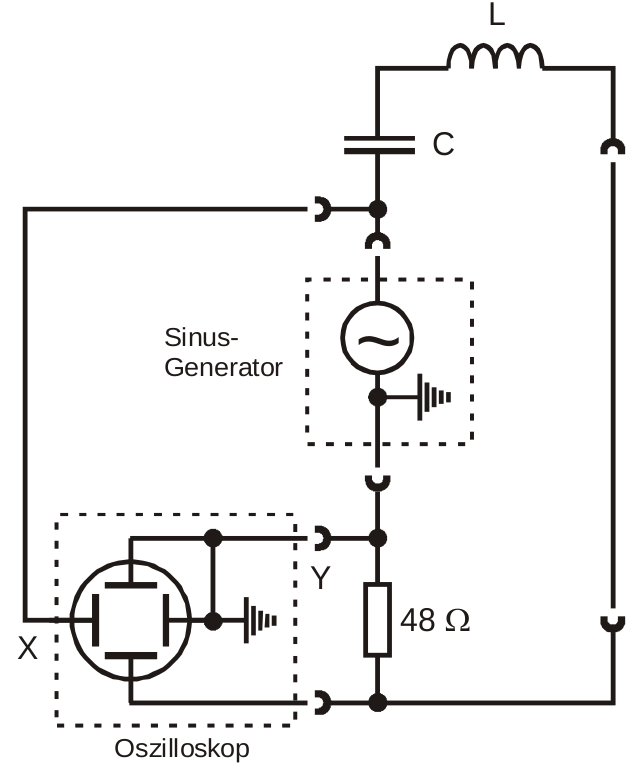
\includegraphics[width = 4cm]{pics/aufbau_resonanzfrequenz.png}
  \caption{Aufbau zur Bestimmung der Resonanzfrequenz \cite{anleitung355}}
  \label{fig: resonanzfrequenz}
\end{figure}


\begin{figure}
  \centering
  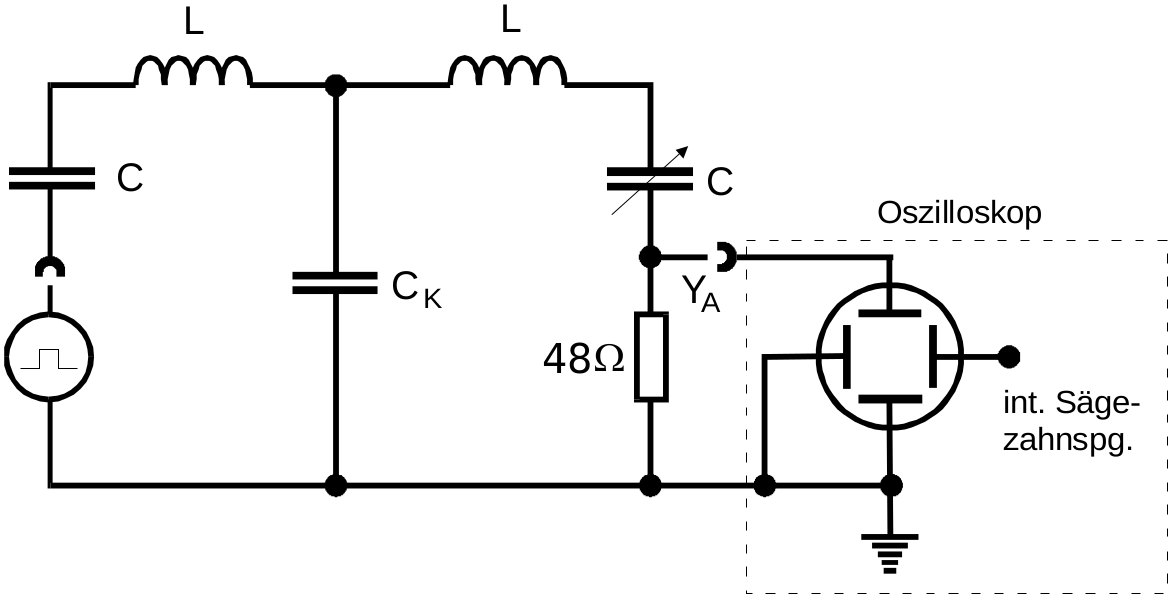
\includegraphics[width = 8cm]{pics/aufbau_schwebung.png}
  \caption{Aufbau zur Untersuchung der Schwebungsvorgänge \cite{anleitung355}}
  \label{fig: schwebung}
\end{figure}
